%%%%%%%%%%%%%%%%%%%%%%%%%%%%%%%%%%%%%%%%%%%%%%%%%%%%%%%%%%%%%%%%%%%%%%%%%%%%%%%%%%%%%%%%%%%%%%%%%%%%%%%%%%%%%%%%%%%%%%%%%%%%%%%%%%%%%%%%%%%%
%%%%%%%%%%%%%%%%%%%%%%%%%%%%%%%%%%%%%%%%%%%%%%%%%%%%%%%%%%%%%%%%%%%%%%%%%%%%%%%%%%%%%%%%%%%%%%%%%%%%%%%%%%%%%%%%%%%%%%%%%%%%%%%%%%%%%%%%%%%%
% Dies ist ein Kommentar, er wird bei der pdf-Erzeugung ignoriert.


% Dies ist eine LaTex-Vorlage für den Gebrauch im Physikalischen Praktikum I und ist als Hilfestellung zu verstehen, falls keine LaTex-Kenntnisse vorhanden sind. Einige nötige und nützliche Pakete sind bereits eingebunden und die Kapitel (\section) angelegt. Die Kapitel beinhalten teilweise Beispiele wie die Darstellung von Grafiken/Tabellen oder mathematischen Formeln sowie Referenzen/Zitationen. Nach den nun folgenden Paketeinbindungen und Definitionen können die Namen der Verfasser, der Versuchsname usw. eingegeben werden. 


%%%%%%%%%%%%%%%%%%%%%%%%%%%%%%%%%%%%%%%%%%%%%%%%%%%%%%%%%%%%%%%%%%%%%%%%%%%%%%%%%%%%%%%%%%%%%%%%%%%%%%%%%%%%%%%%%%%%%%%%%%%%%%%%%%%%%%%%%%%%
%%%%%%%%%%%%%%%%%%%%%%%%%%%%%%%%%%%%%%%%%%%%%%%%%%%%%%%%%%%%%%%%%%%%%%%%%%%%%%%%%%%%%%%%%%%%%%%%%%%%%%%%%%%%%%%%%%%%%%%%%%%%%%%%%%%%%%%%%%%%
\documentclass[a4paper,12pt,bibtotocnumbered]{scrartcl}

\usepackage[utf8]{inputenc} %Codierung des LaTeX-Dokumentes. Auf Windows-Maschinen ist statt utf8 auch ANSIC als Codierung möglich, aber unnötig, da utf8 in jeder Hinsicht besser als ANSI ist. Bei Linux: latin1 als Codierung, auf MacOS X: applemac
\usepackage[T1]{fontenc}
\usepackage[ngerman]{babel} %Deutsche Zeichen- und Umbruchsetzung
\usepackage{amsmath, amssymb,amsfonts} %AMS-TeX-Pakete. Nötig für die Definition der Mathematik-Umgebung
\usepackage{graphicx} %Nötig, um Grafiken einbinden zu können
\usepackage[bookmarks,colorlinks=true]{hyperref} %Mittels hyperref lassen sich hyperlinks innerhalb des PDF-Dokumentes benutzen. Beispiel: Mausklick im Inhaltsverzeichnis auf ein Kapitel führt zum automatischen Sprung in dieses Kapitel
\usepackage{geometry}
\usepackage{float}
%Ein Paket, mit dem sich ohne Probleme mehrseitige PDF-Dokumente ohne \includegraphics-Rumgemache einbinden lassen. Befehl: \includepdf[pages=a-b]{PDFfile.pdf}. Einzelne Seiten, oder auch alle Seiten (Option pages=-) können angewählt werden
%Wenn keine Option angegeben wird, gilt pages=1!
\usepackage[final]{pdfpages}
\usepackage{framed, color} %Framed: Paket, mittels dessen ein Rahmen um einen Bereich definiert werden kann. Color: Lässt Farbdarstellung in Schrift, Hintergrund etc. zu
\usepackage{scrlayer-scrpage} %Header für die KOMA-script -Klasse
\usepackage{siunitx} %Ein schönes Paket, um Einheiten und physikalische Größen richtig zu setzen. Z.B.  \SI{2}{\kilo\gram\per\meter\squared}
\usepackage[square,numbers]{natbib}
\usepackage{subfigure} %Mehrere Bilder in einer Figure-Umgebung
\usepackage{lipsum}  
\usepackage{setspace}
\usepackage{booktabs}
\usepackage{csquotes}
\MakeOuterQuote{"}


%siunitx-Konfiguration. Damit werden die richtigen Font-Einstellungen erkannt (also beispielsweise fett, kursiv etc.) und damit  ebenfalls die deutsche Zeichensetzung, insbesondere Trennungszeichen, benutzt werden. 
%Ebenso wird bei SIrange das "`to"' in "`bis"' umgewandelt, bei SIlist das "`and"' in "`und"'
\sisetup{detect-weight=true, detect-family=true,locale=DE,range-phrase={\,bis\,},list-final-separator ={\,\linebreak[0] \text{und}\,},separate-uncertainty=true,per-mode = symbol-or-fraction}
%\SI[per-mode = fraction]{1}{\meter\per\second} erzwingt auch im Fließtext die Bruchdarstellung.
\DeclareSIUnit\curie{Ci}%Zusätzliche Einheit definieren

%Hyperlinks-Setup
\hypersetup{
	colorlinks,
	linktoc=all,
	citecolor=black,
	filecolor=black,
	linkcolor=black,
	urlcolor=black
}

\numberwithin{equation}{section} % Die Nummerierung von Gleichungen bekommt die jeweilige Section-Nummer als Präfix

\setlength{\parindent}{0 mm} %Einrücktiefe von neuen Absätzen
\setlength{\parskip}{2 mm} %Abstand von Absätzen



\pagestyle{scrheadings}%Kopf und Fußzeilen
\ohead{\textbf{\VERSUCHSNR}} %Header oben links auf linker Seite (ungerade Seitenzahl) und oben rechts auf rechter Seite (gerade Seitenzahl), beinhaltet gruppennummer und Versuchskürzel. Im Fall eine einseitigen Dokuments: Header oben rechts
\ihead{113469b Praktikum 3D-Druck} %Header oben rechts auf linker Seite und oben links auf rechter Seite. Beinhaltet die Namen der Verfasser. Im Fall eine einseitigen Dokuments: Header oben links!
\ofoot{\thepage} %Footer unten links auf linker und unten rechts auf rechter Seite, enthält die jeweilige Seitenzahl. Im Fall eines einseitigen Elements: Footer unten rechts!
\cfoot{\empty} %Mittig unten im Footer soll nichts eingetragen werden 
\ifoot{\VerfasserEINS} %Footer unten rechts auf linker und unten links auf rechter Seite. Hier ebenfalls leer.


%%%%%%%%%%%%%%%%%%%%%%%%%%%%%%%%%%%%%%%%%%%%%%%%%%%%%%%%%%%%%%%%%%%%%%%%%%%%%%%%%%%%%%%%%%%%%%%%%%%%%%%%%%%%%%%%%%%%%%%%%%%%%%%%%%%%%%%%%%%%

% Hier können die individuellen Anpassungen vorgenommen werden, die sich auf das Titelblatt und die Kopfzeilen auswirken.

\newcommand{\VERSUCHSDATUM}{06.04.2022}
\newcommand{\PROTOKOLLDATUM}{\today}

\newcommand{\VerfasserEINS}{Hannes Frey}
\newcommand{\MatNoEINS}{39311}
\newcommand{\StudiengangEINS}{MI7}
\newcommand{\SemesterEINS}{6. Semester}
\newcommand{\MailEINS}{hf018@hdm-stuttgar.de}

\newcommand{\VerfasserZWEI}{Verfasser 2}
\newcommand{\MatNoZWEI}{Matrikelnummer 2}
\newcommand{\StudiengangZWEI}{Technologiemanagement}

\newcommand{\BETREUER}{Karl Schaschek}
\newcommand{\WORTZAHL}{1000}
\newcommand{\GRUPPENNR}{Z-999}

\newcommand{\VERSUCHSNR}{Übung 03}
\newcommand{\VERSUCHSNAME}{Einfluss der Schichtdicke auf den maximalen Überhangwinkel}

%%%%%%%%%%%%%%%%%%%%%%%%%%%%%%%%%%%%%%%%%%%%%%%%%%%%%%%%%%%%%%%%%%%%%%%%%%%%%%%%%%%%%%%%%%%%%%%%%%%%%%%%%%%%%%%%%%%%%%%%%%%%%%%%%%%%%%%%%%%%
% Hier beginnt die Titelseite

\begin{document}
\thispagestyle{empty}


\begin{titlepage}

\begin{center}
\Huge{\textbf{\VERSUCHSNR\ – \VERSUCHSNAME}}\\% \Huge \huge \Large \normalsize \Small usw. bestimmt die Schriftgröße.
\vspace{10mm}% Abstand
\Large{Protokoll zum Versuch des 3D-Druck Praktikums 113469  % von \\ \textbf{\VerfasserEINS\;}
}\\
\vspace{10mm} 
\Large{Hochschule der Medien Stuttgart}\\
\end{center}
\vspace{1cm}
\begin{center}
\begin{tabular}{ll}
\large{Verfasser:}		& \large{\VerfasserEINS\;(\StudiengangEINS, \SemesterEINS),} \\ 
						& \large{\MailEINS}, \\
 						& \large{\MatNoEINS} \\
% 						\vspace{0cm}\\
%						& \large{\VerfasserZWEI\;(\StudiengangZWEI),} \\
%						& \large{\MatNoZWEI} \\
						\vspace{0cm}\\
%\large{Gruppennummer:}	& \large{\GRUPPENNR} \\
\vspace{0cm}\\
\large{Versuchsdatum:}	& \large{\VERSUCHSDATUM} \\
\vspace{0cm}\\
\large{Betreuer:}		& \large{\BETREUER} \\
\vspace{0cm}\\
\large{Wortzahl:}		& \large{\WORTZAHL}
\end{tabular}
\end{center}
\vspace{65mm}

\begin{center}
Stuttgart, den \PROTOKOLLDATUM
\end{center}

\end{titlepage}


\thispagestyle{empty}
%%%%%%%%%%%%%%%%%%%%%%%%%%%%%%%%%%%%%%%%%%%%%%%%%%%%%%%%%%%%%%%%%%%%%%%%%%%%%%%%%%%%%%%%%%%%%%%%%%%%%%%%%%%%%%%%%%%%%%%%%%%%%%%%%%%%%%%%%%%%%%%%
%Mittels des untenstehenden einfachen Befehls wird ein Inhaltsverzeichnis angelegt. LaTeX erstellt das Inhaltsverzeichnis völlig automatisch anhand der Überschriften für Kapitel, Unterkapitel etc. Das Dokument muss
%unter Umständen zweimal neu gesetzt werden, damit Änderungen in den Überschriften auch im Inhaltsverzeichnis auftauchen!
%%%%%%%%%%%%%%%%%%%%%%%%%%%%%%%%%%%%%%%%%%%%%%%%%%%%%%%%%%%%%%%%%%%%%%%%%%%%%%%%%%%%%%%%%%%%%%%%%%%%%%%%%%%%%%%%%%%%%%%%%%%%%%%%%%%%%%%%%%%%%%%%
\tableofcontents 
%%%%%%%%%%%%%%%%%%%%%%%%%%%%%%%%%%%%%%%%%%%%%%%%%%%%%%%%%%%%%%%%%%%%%%%%%%%%%%%%%%%%%%%%%%%%%%%%%%%%%%%%%%%%%%%%%%%%%%%%%%%%%%%%%%%%%%%%%%%%%%%%
\clearpage %Neue Seite, davor werden alle noch ausstehenden Grafiken/Tabellen platziert.


\renewcommand{\thepage}{\arabic{page}}
\setcounter{page}{1}


%%%%%%%%%%%%%%%%%%%%%%%%%%%%%%%%%%%%%%%%%%%%%%%%%%%%%%%%%%%%%%%%%%%%%%%%%%%%%%%%%%%%%%%%%%%%%%%%%%%%%%%%%%%%%%%%%%%%%%%%%%%%%%%%%%%%%%%%%%%%
%%%%%%%%%%%%%%%%%%%%%%%%%%%%%%%%%%%%%%%%%%%%%%%%%%%%%%%%%%%%%%%%%%%%%%%%%%%%%%%%%%%%%%%%%%%%%%%%%%%%%%%%%%%%%%%%%%%%%%%%%%%%%%%%%%%%%%%%%%%%
%%%%%%%%%%%%%%%%%%%%%%%%%%%%%%%%%%%%%%%%%%%%%%%%%%%%%%%%%%%%%%%%%%%%%%%%%%%%%%%%%%%%%%%%%%%%%%%%%%%%%%%%%%%%%%%%%%%%%%%%%%%%%%%%%%%%%%%%%%%%

% Abbildungsverzeichnis
\listoffigures
\addcontentsline{toc}{section}{Abbildungsverzeichnis}

% Tabellenverzeichnis
%\listoftables
%\addcontentsline{toc}{section}{Tabellenverzeichnis}

\newpage
\onehalfspacing 

% Die erste eckige Klammer ist optional, die darin angegebene Bezeichnung steht im Inhaltsverzeichnis anstelle des hinteren (längeren) Namens.
\section[Einführung]{Einführung und Versuchsziel}

Ziel des Versuchs ist es, die Abhängigkeit von Schichtdicke und Qualität von Überhangdrucken zu analysieren. Hierfür wird das zur Verfügung gestellte Objekt mit den Schichtdicken 0.2 mm, 0.1 mm sowie 0.07 mm gedruckt und die Überhänge miteinander vergleichen. Ebenso wird ein Druck mit Unterstützungsmaterial für zu große Überhangwinkel erstellt.

\section[Verwendete Geräte, Materialien und Hilfsmittel]{Verwendete Geräte, Materialien und Hilfsmittel}

Zur Versuchsdurchführung wurde ein 3D Drucker der Marke Prusa, Modell i3 MK3S+ mit Filament des Typs PLA verwendet. 

Zur Protokollerstellung kam \LaTeX\;zum Einsatz, Screenshots des PrusaSlicers konnten mit der Windows eigenen Lösung erstellt werden. Bilder des gedruckten Objekts wurden mit einem Smartphone Marke Google erstellt, ein 2D-Scan mit einem Brother MFC-9332CDW Drucker.

\newpage

\section[Versuchsdurchführung]{Versuchsdurchführung}

Zur Vorbereitung wurde das Programm PrusaSlicer gestartet und das zur Verfügung gestellte Modell (siehe Abbildung \ref*{model}) Vier mal eingefügt. 


\begin{figure}[H]
\centerline{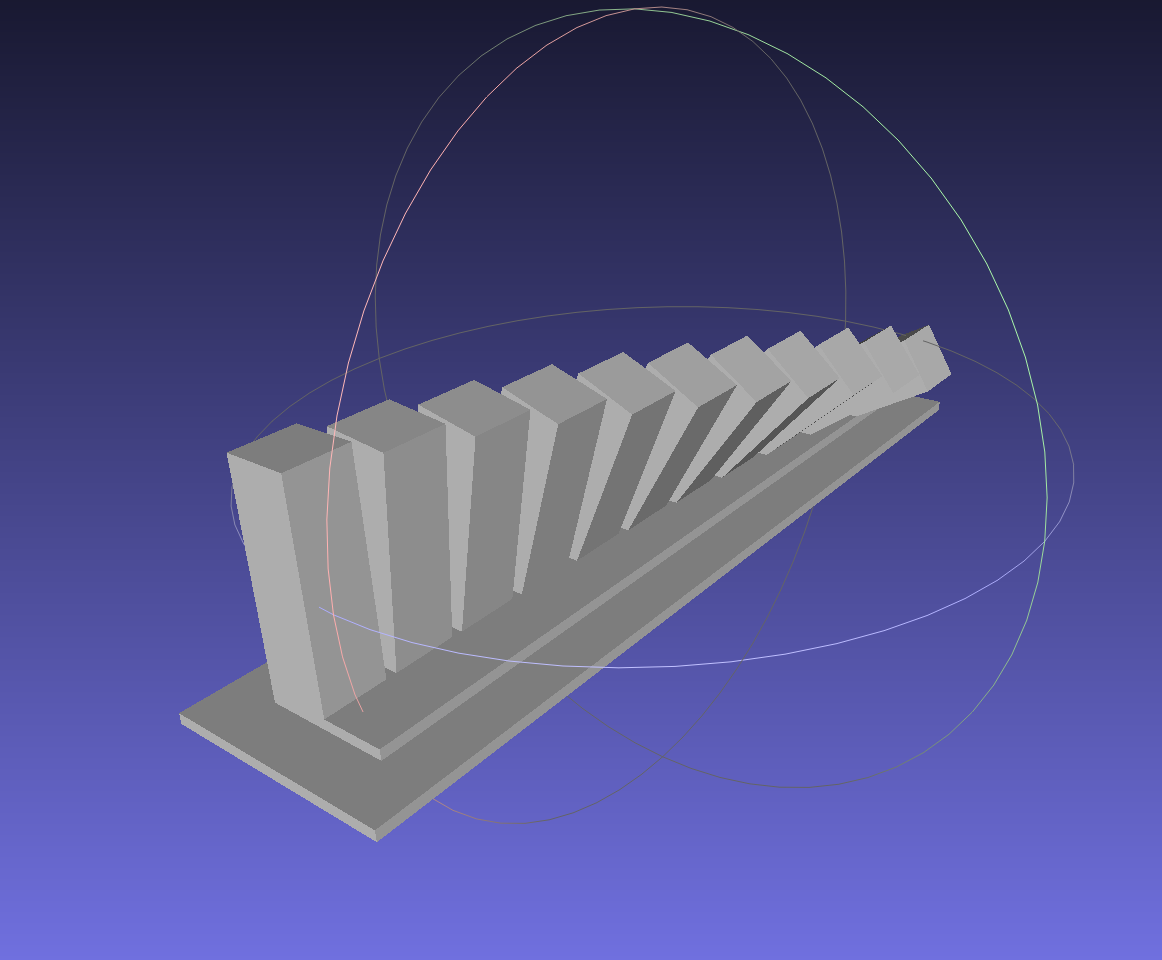
\includegraphics[width=200px]{./images/model.png}}
\caption{MeshLab - Ansicht des Modells}
\label{model}
\end{figure}

Über die in Abbildung \ref*{layerheight} zu sehende Einstellungsoption lassen sich die Schichtdicken unterschiedlicher Objekte je Objekt individuell einstellen und so in einem Druck alle Schichtdicken erreichen.

\begin{figure}[H]
\centerline{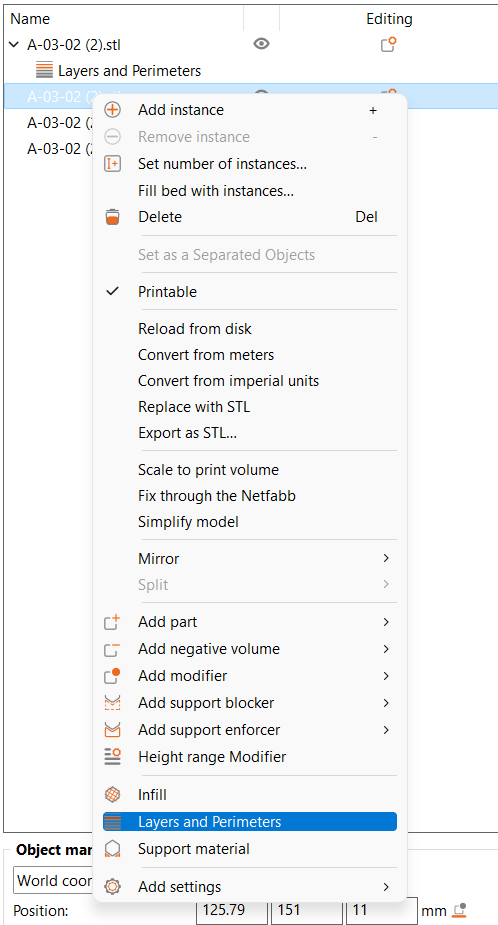
\includegraphics[width=200px]{./images/lyerheight.png}}
\caption{PrusaSlicer - Kontextmenü eines eingeladenen Modells}
\label{layerheight}
\end{figure}

Zu sehen sind diese unterschiedlichen Schichtdicken in Abbildung \ref*{slice_now}. Das Model hinten links hat dabei die Schichtdicke von 0.2 mm, vorne links 0.07 mm. Das dritte Objekt ohne Stützstrukturen die Dicke 0.1 mm, und das letzte Model wurde ebenso mit einer Schichtstärke von 0.2 mm gedruckt.
			
\begin{figure}[H]
\centerline{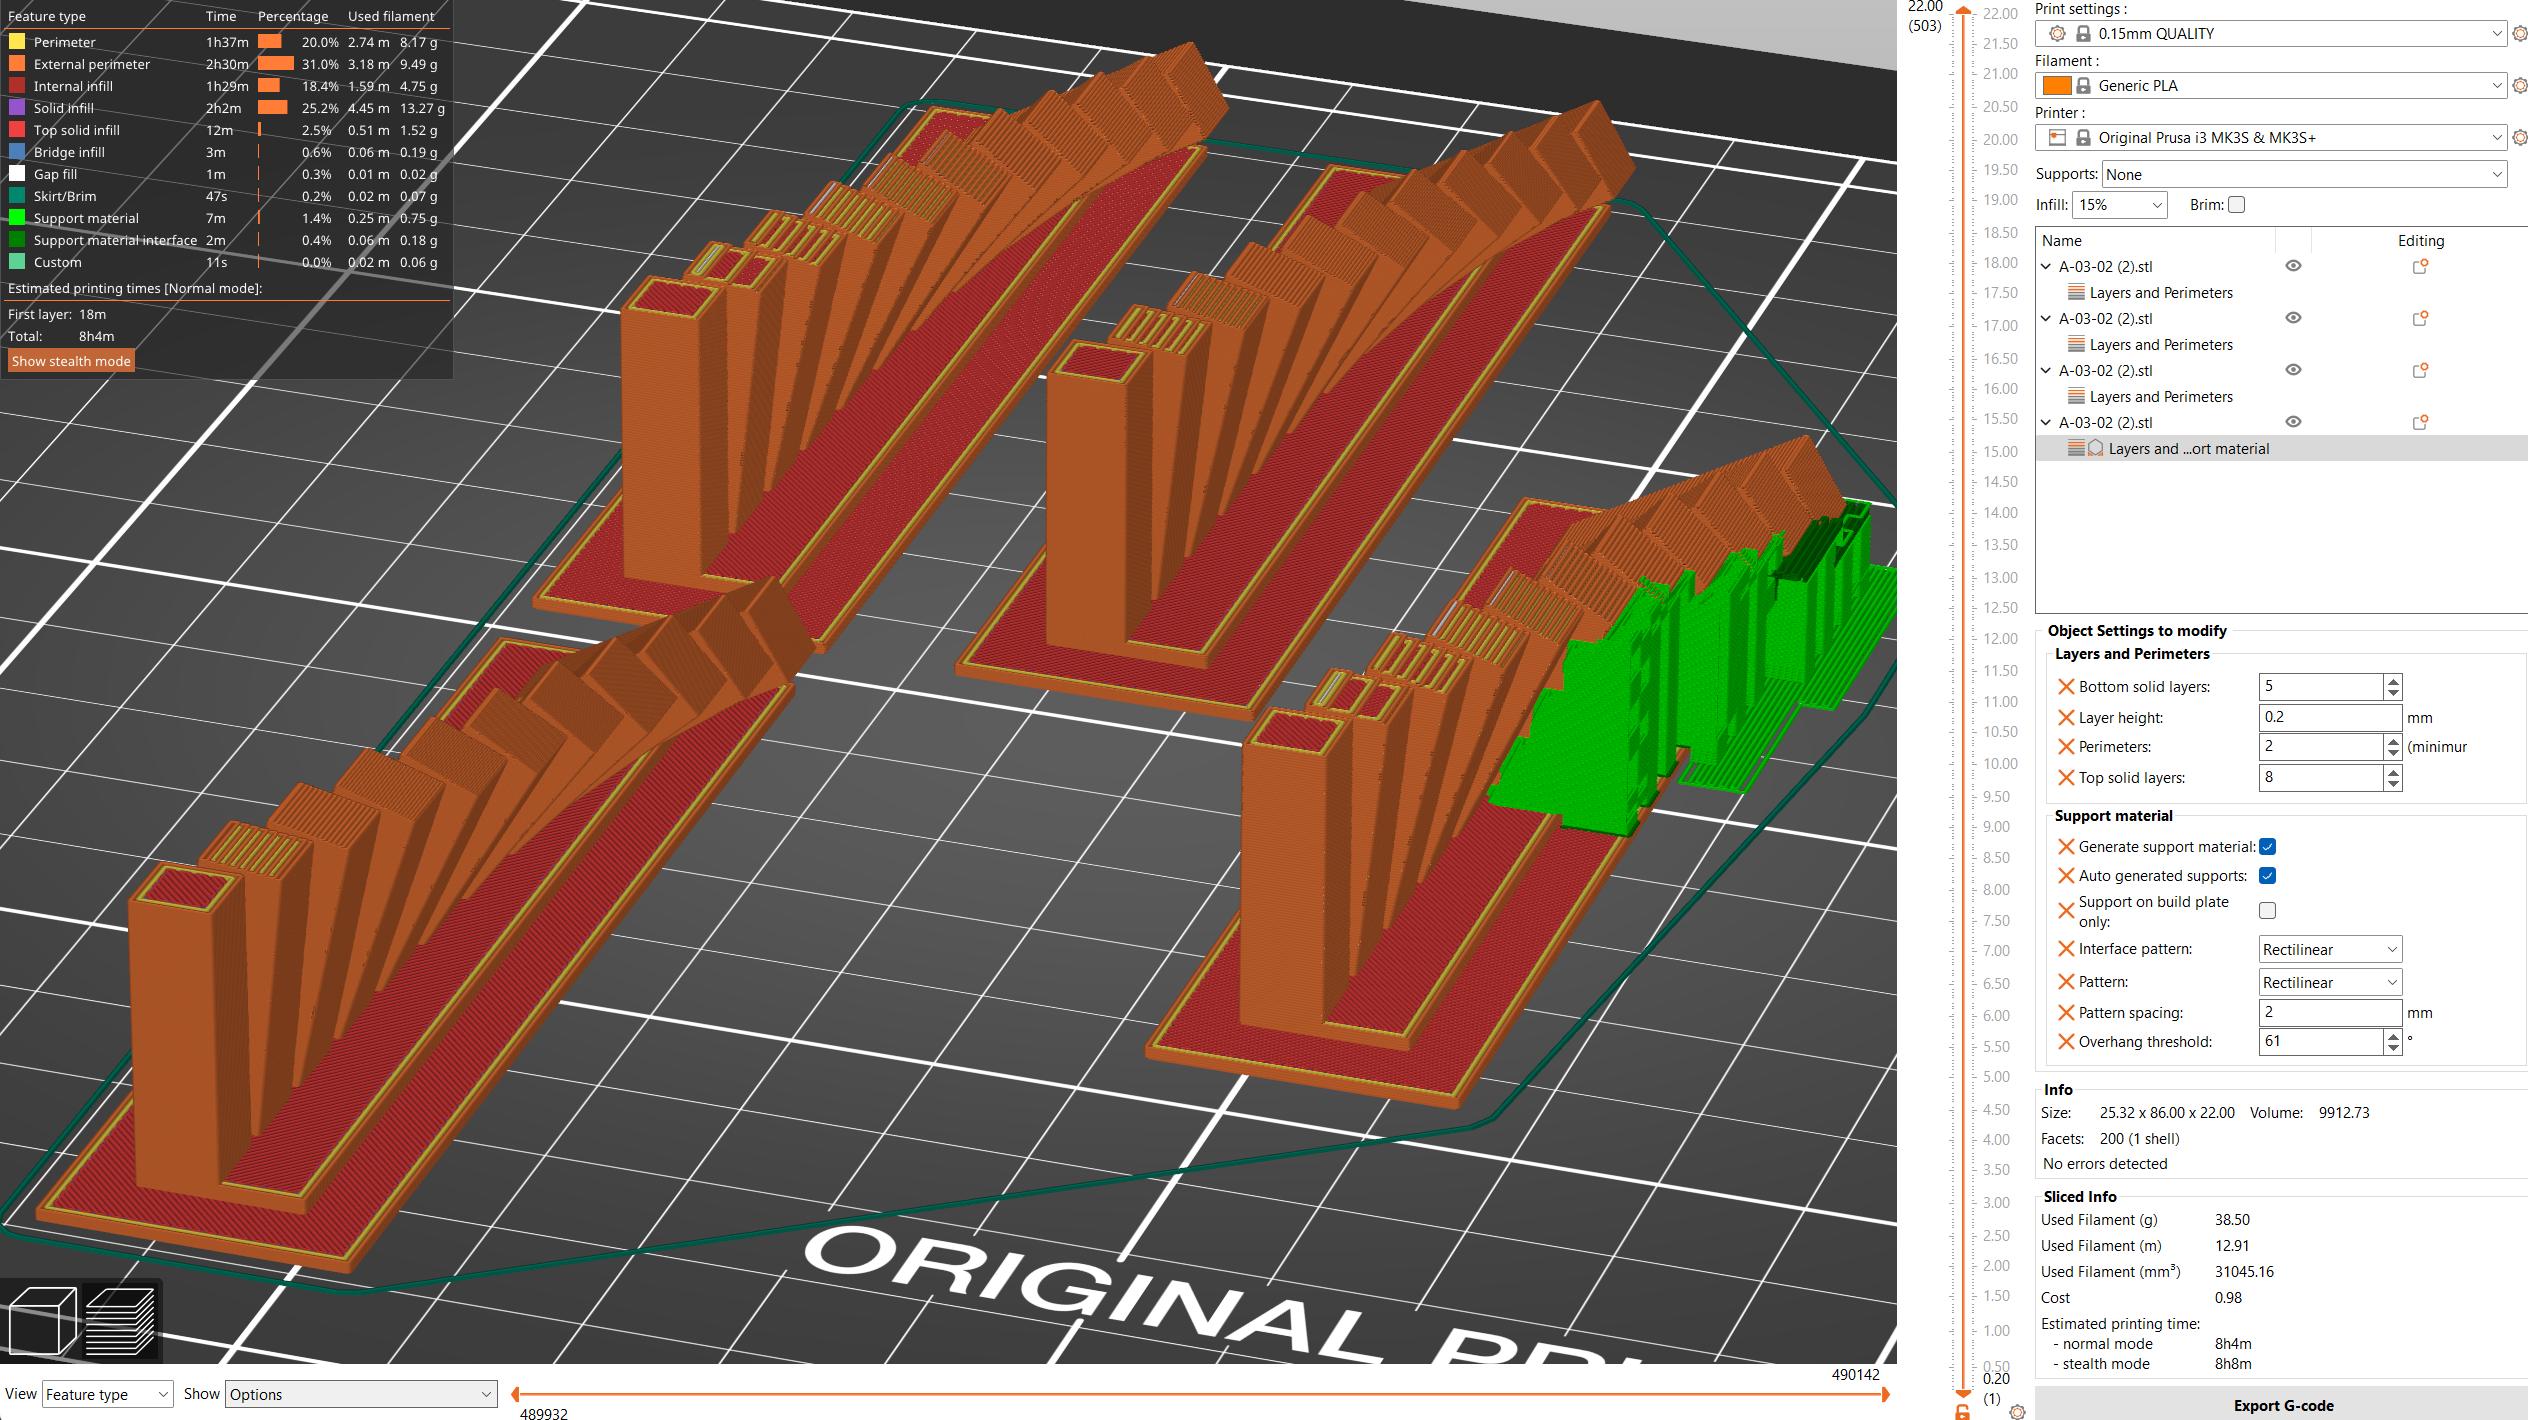
\includegraphics[width=380px]{./images/prusa.png}}
\caption{PrusaSlicer - Übersicht der Druckobjekte}
\label{slice_now}
\end{figure}

\section[Auswertung und Analyse]{Auswertung und Analyse}
Die Auswertung gestaltete sich als anspruchsvoller als gedacht, da sich die Druckqualität nur minimal von Objekt zu Objekt unterschied. Als Vorüberlegung erstellte ich mir in Abbildung \ref*{schaubild} zu sehende Grafik. Demnach sollten aufgrund der deutlich höheren Überlappungsfläche Überhänge mit geringerer Schichtdicke deutlich besser zu drucken sein.

\begin{figure}[H]
\centerline{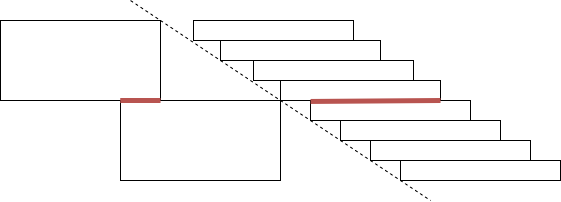
\includegraphics[width=250px]{./images/layerheights.drawio.png}}
\caption{Überlappungen von Überhängen unterschiedlich hoher Druckschichten}
\label{schaubild}
\end{figure}

Betrachtet man jedoch die gedruckten Modelle entsteht die Grafik Abbildung \ref*{abhängigkeit}, welche genau das Gegenteil aufzeigt. Hier wird deutlich, dass je höher die Schichtdicke, desto größere Überhangwinkel können mit akzeptabler Qualität geduckt werden. Diese Unterschiede können auch in Abbildung \ref*{druck1} - \ref*{druck4} gesehen werden.

\begin{figure}[H]
\centerline{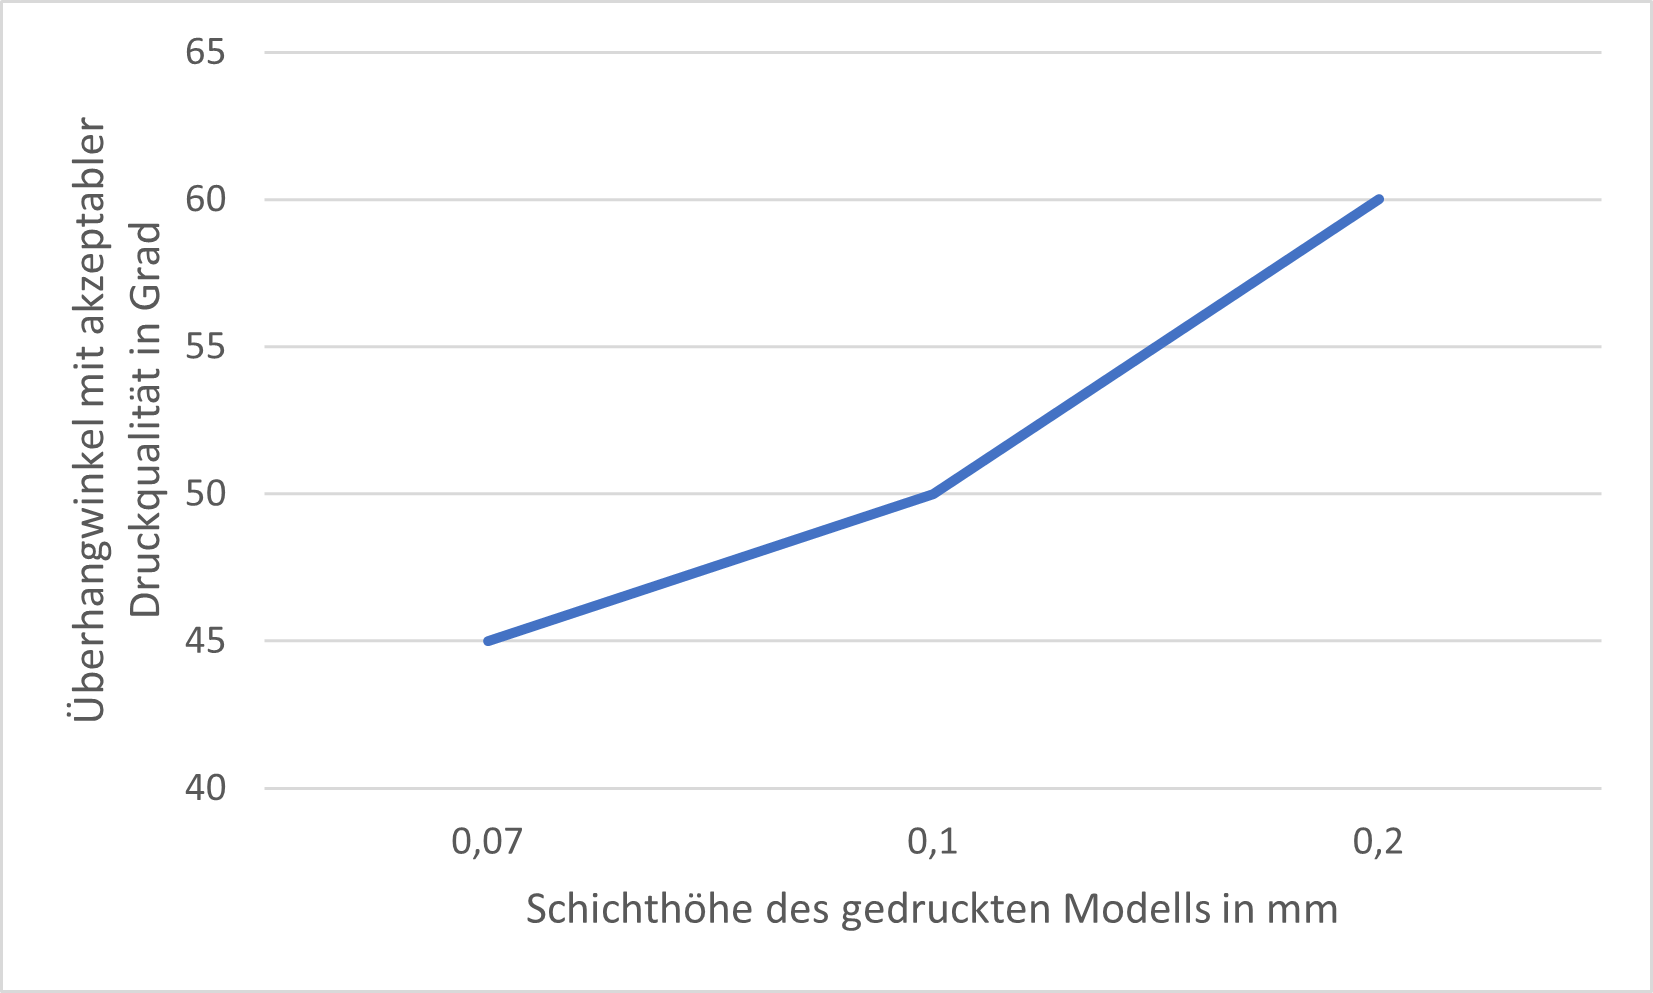
\includegraphics[width=250px]{./images/diagramm.png}}
\caption{Abhängigkeit Schichtdicke - Überhangwinkel mit akzeptabler Qualität}
\label{abhängigkeit}
\end{figure}

\begin{figure}[H]
\centerline{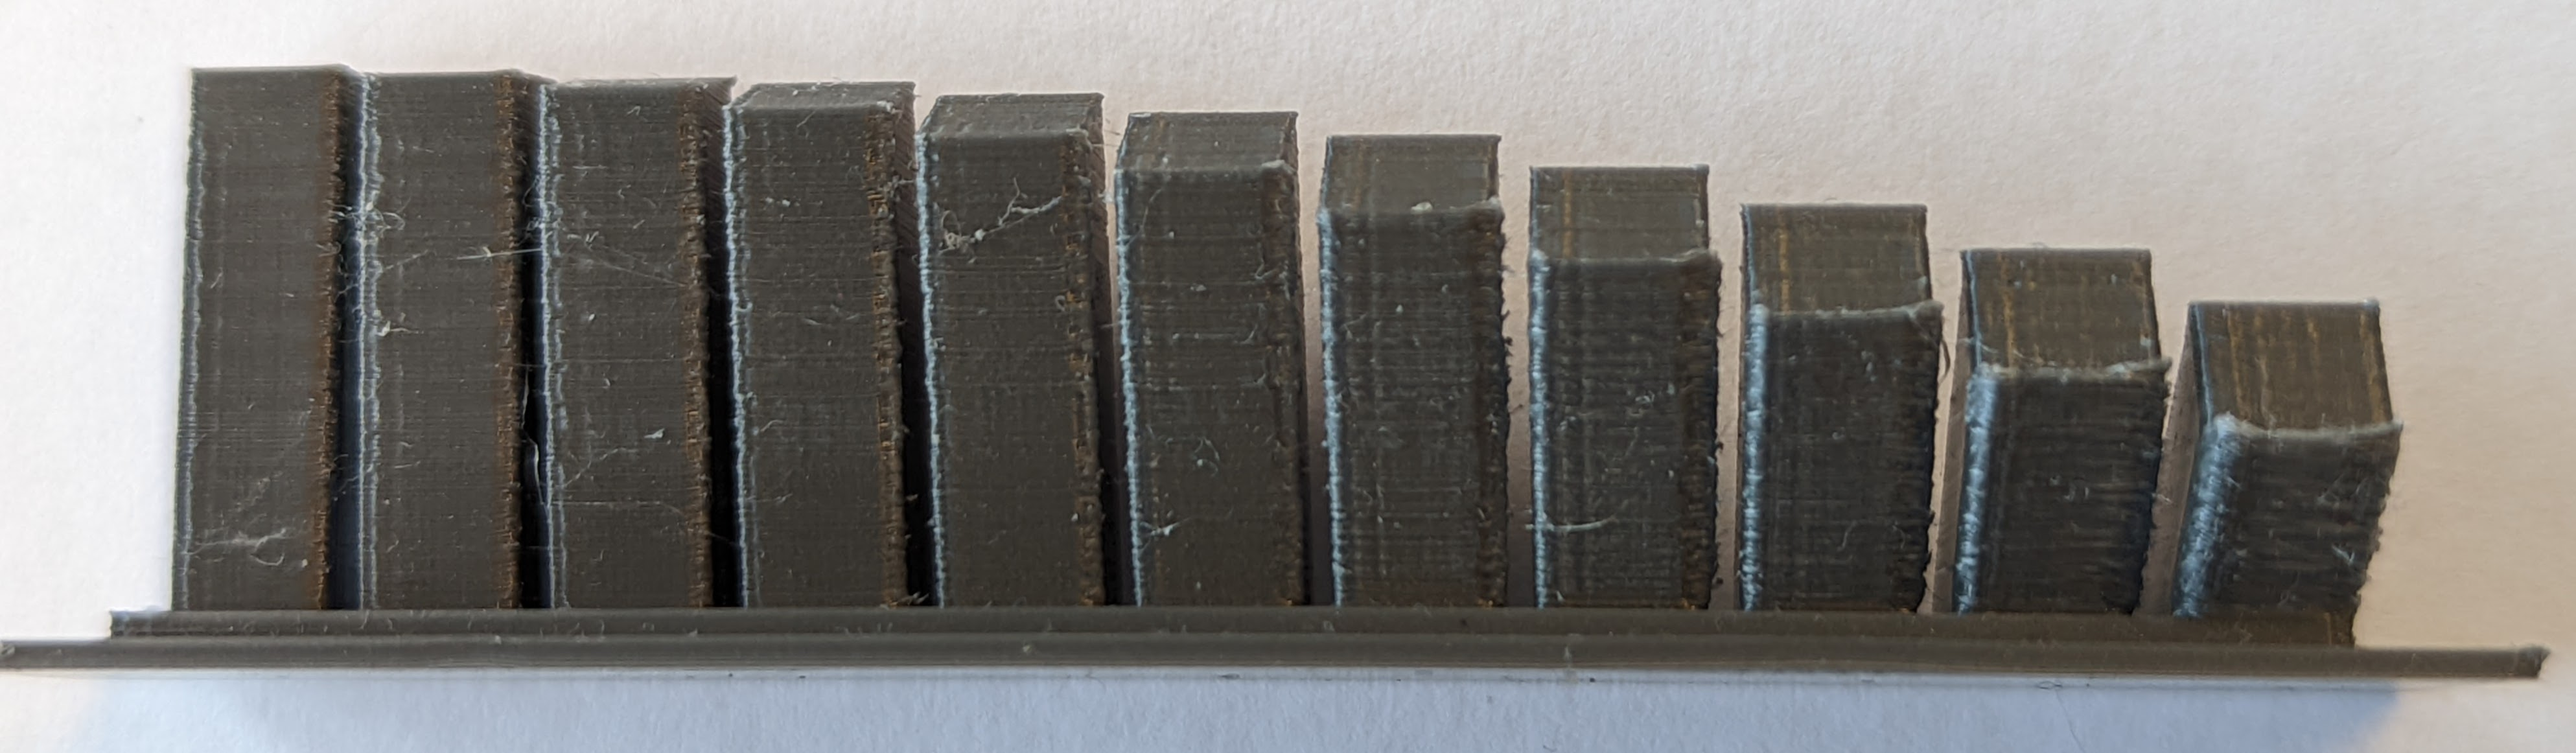
\includegraphics[width=250px]{./images/007.jpg}}
\caption{Front des gedruckten Objekts - 0.07 mm Schichtdicke}
\label{druck1}

\end{figure}
\begin{figure}[H]
\centerline{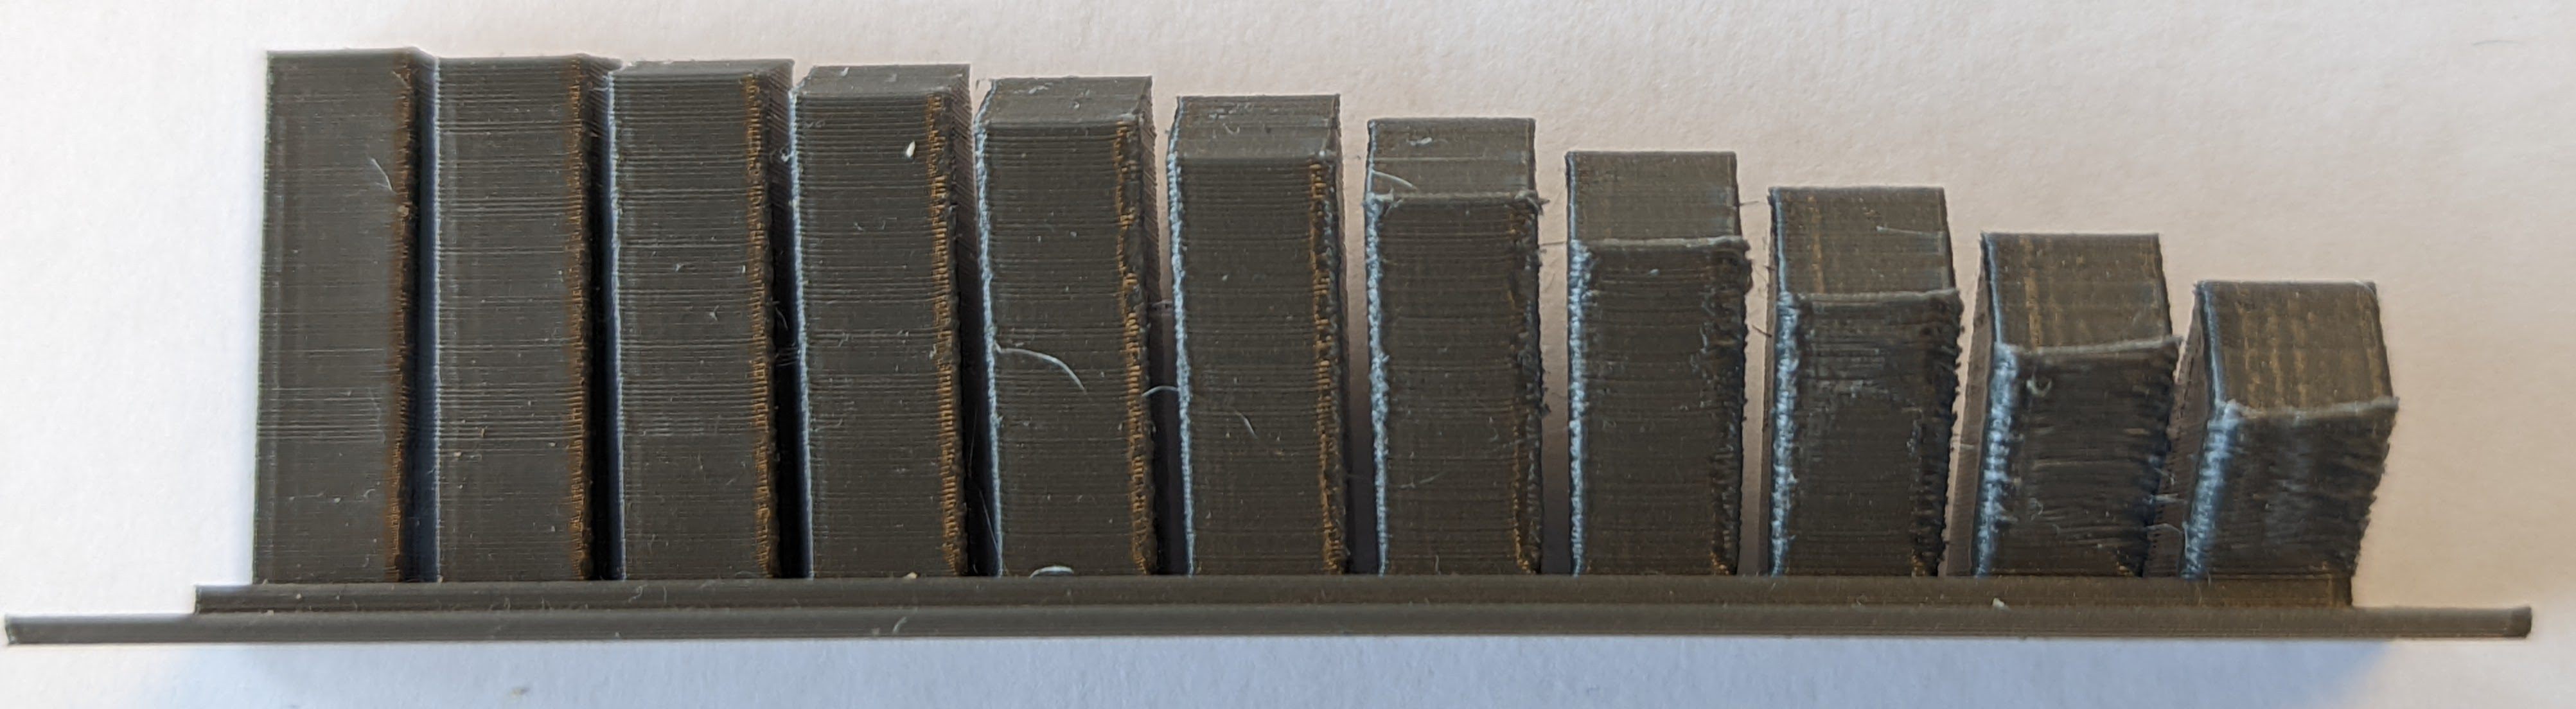
\includegraphics[width=250px]{./images/010.jpg}}
\caption{Front des gedruckten Objekts - 0.10 mm Schichtdicke}
\label{druck2}
\end{figure}

\begin{figure}[H]
\centerline{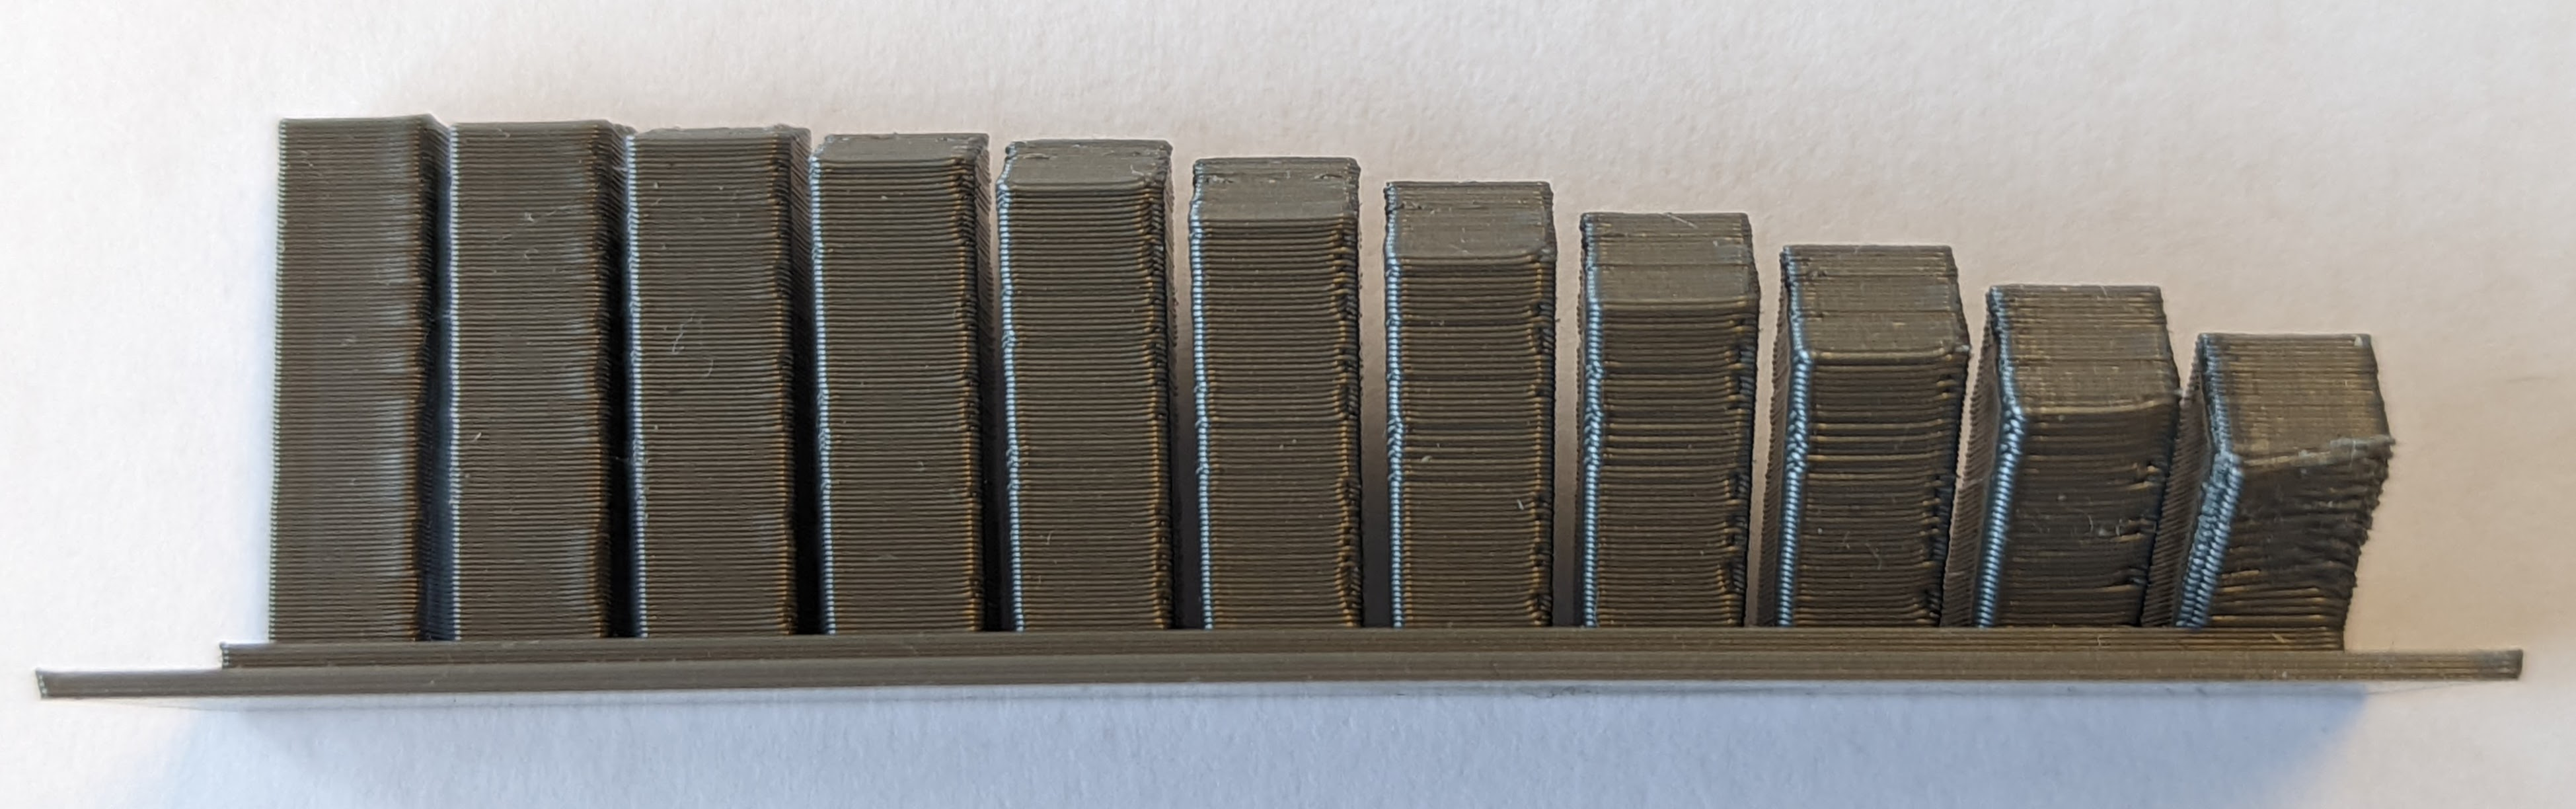
\includegraphics[width=250px]{./images/020.jpg}}
\caption{Front des gedruckten Objekts - 0.20 mm Schichtdicke}
\label{druck3}
\end{figure}

\begin{figure}[H]
\centerline{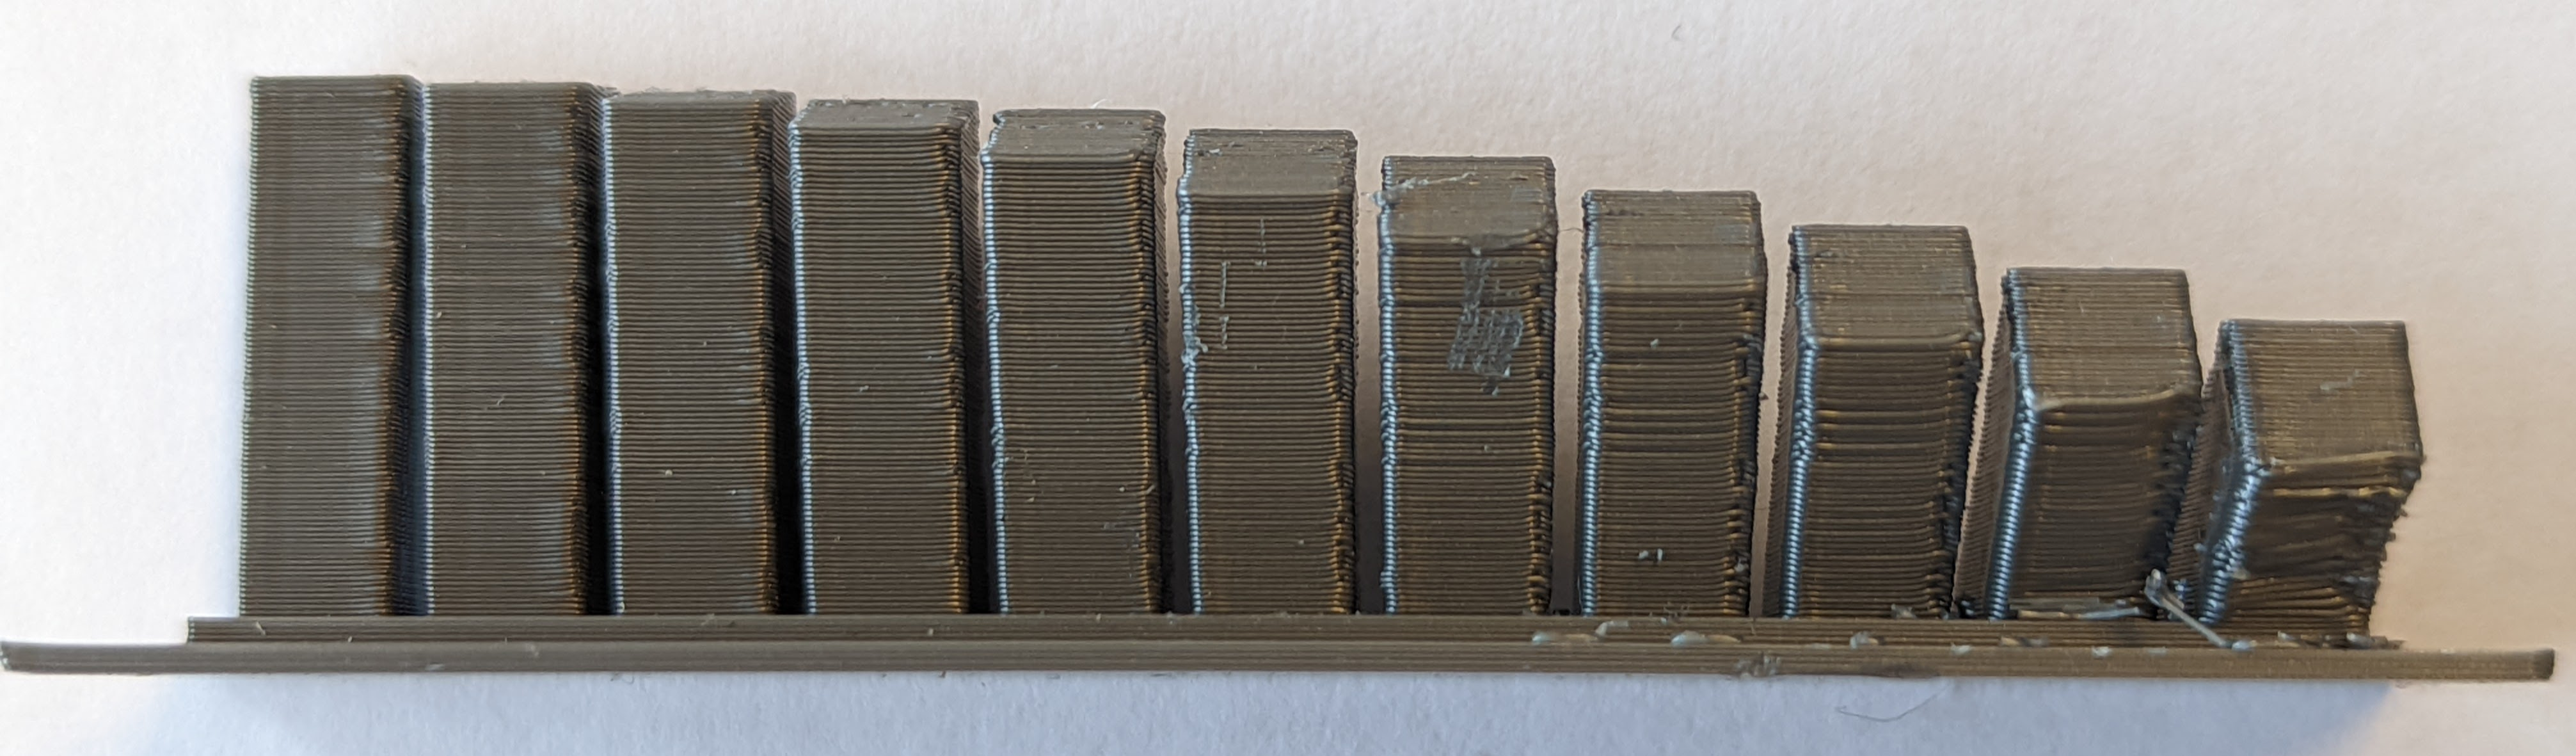
\includegraphics[width=250px]{./images/020_sup.jpg}}
\caption{Front des gedruckten Objekts - 0.20 mm Schichtdicke und entferntes Unterstützungsmaterial}
\label{druck4}
\end{figure}

Eine Erklärung hierfür könnten die unterschiedlichen Abkühlverhalten der Schichtdicken sein. Ist ein Layer sehr dünn, so besteht die Möglichkeit, dass sich dieser bei einer erneuten Überfahrung der Düse eine Schicht weiter so stark erwärmt, dass es erneut zu einer Verflüssigung kommt. Diese zwei flüssigen Schichten kühlen dann unterschiedlich schnell ab, wodurch es zu einer Verformung kommt und was sich negativ auf die Druckqualität auswirkt.

Die Qualität des Druckes mit Unterstützungsmaterial ist nur marginal besser, da auch das Hilfsmaterial seine Spuren hinterlassen hat. Ebenso ließ sich dieses nicht einfach entfernen, was zu zusätzlichen Spuren am Objekt geführt hat. Der Sinn hinter Hilfsmaterial ist, bei Überhangdrucken neuen Schichten zusätzliche Stabilität zu bieten. Bei Drucken mit sehr großen solcher Winkel, wie im Extremfall beispielsweise 90 Grad, ist es sicherlich sinnvoll und sogar notwendig mit Unterstützungsmaterial zu drucken. In diesem Fall ist es allerdings nicht notwendig, und macht durch das zusätzliche zu druckende Material den Druck nur länger.

Bezüglich Drucklänge liefert Abbildung \ref*{print_duration} nützliche Informationen. Hier ist das gedruckte Modell mit Unterstützungsstrukturen nicht nennenswert, denn dessen Druckdauer verlängerte sich im Vergleich zum Modell ohne Hilfsmaterial nur um 3 Minuten.


\begin{figure}[H]
	\centerline{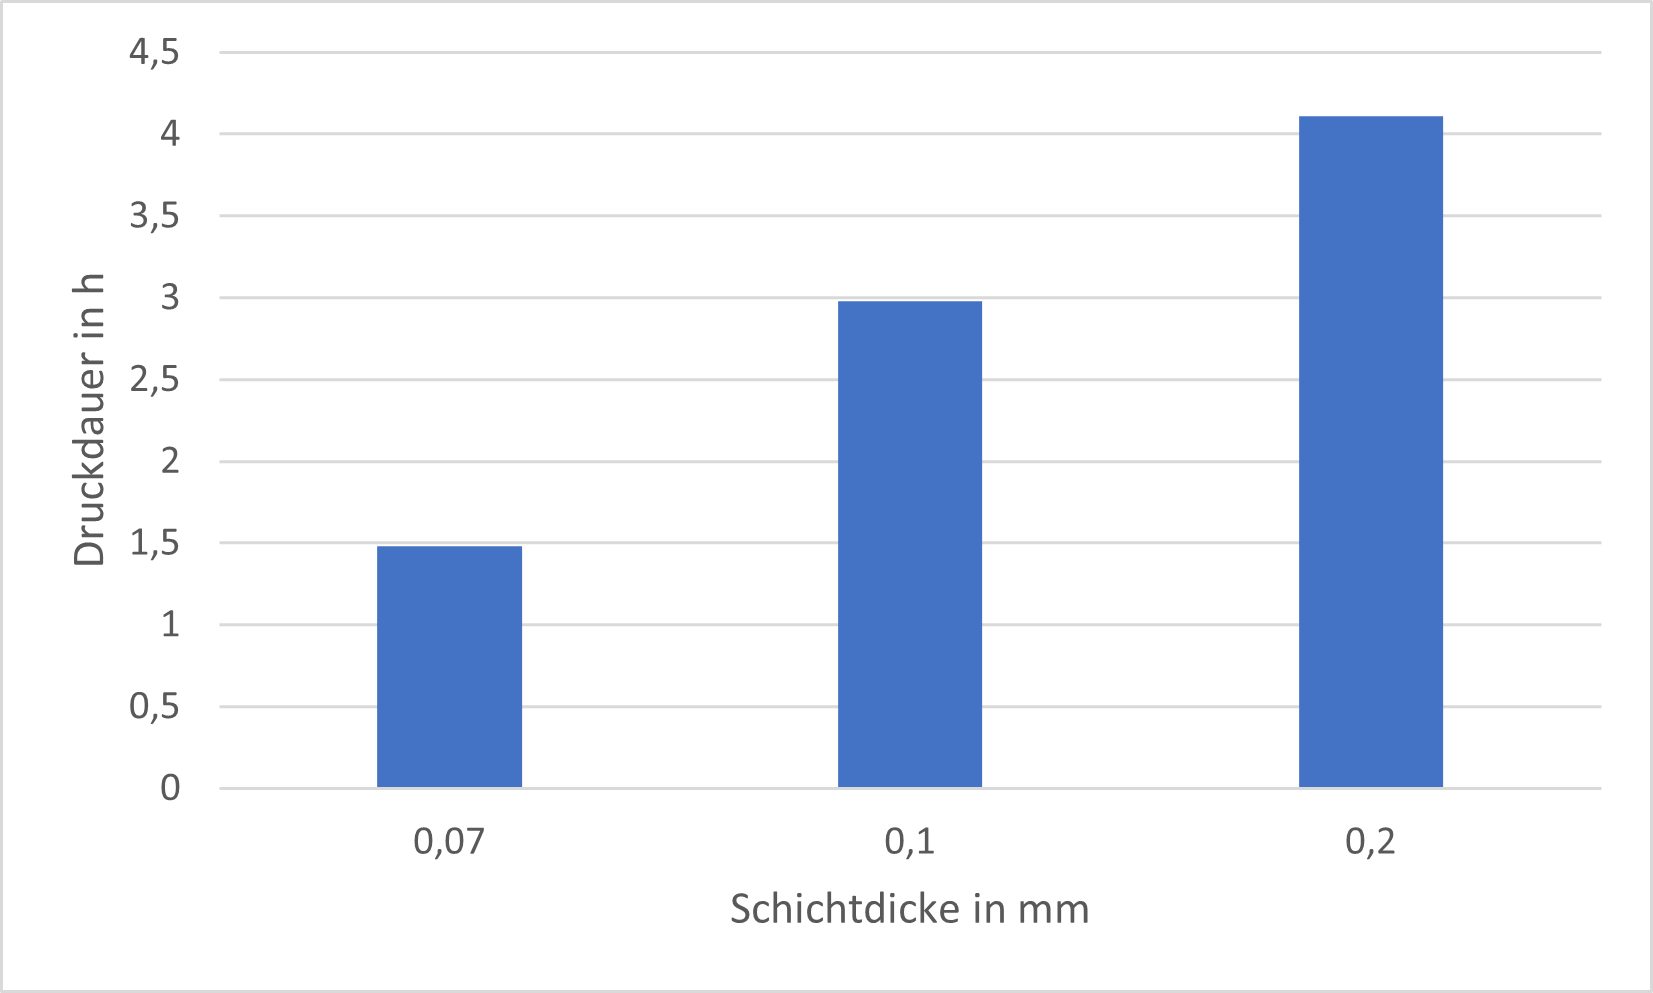
\includegraphics[width=250px]{./images/dauer.png}}
	\caption{Abhängigkeit Schichtdicke - Druckdauer}
	\label{print_duration}
	\end{figure}

Interessant zu sehen ist, dass obwohl sich die Anzahl der Schichten von 0,20 mm zu 0,10 mm Druckeinstellung verdoppelt habt, die Druckdauer nicht doppelt so lang ist. Der Grund hierin liegt höchstwahrscheinlich in den ersten Schichten, die in beiden Fällen besonders langsam gedruckt werden.

%Hier wird eine Quelle zitiert \cite{Quelle}.
\newpage
\begin{thebibliography}{999}
\bibitem{Quelle} Versuchsanleitung zu Versuch 03 (Abgerufen am 09.04.2022) 
\end{thebibliography}

% Für Dokumente mit mehr Referenzen empfiehlt es sich, auf eine separate .bib -Datei umzusteigen, die alle Referenzen enthält. Diese Referenzen können bei den meisten wissenschaftlichen Publikationen direkt über "BibTex-Export" oder ähnliches heruntergeladen werden. Anstelle von \begin{thebibliography}...\bibitem{}..\bibitem{}..\end{thebibliography} muss dann lediglich \bibliography{Dateiname.bib} eingebunden werden.

%\section{Anhang}
%\includepdf[pages=-]{Dateiname.pdf}


\end{document}